\documentclass{standalone}
\usepackage{tikz}
\usetikzlibrary{patterns, positioning}

\begin{document}
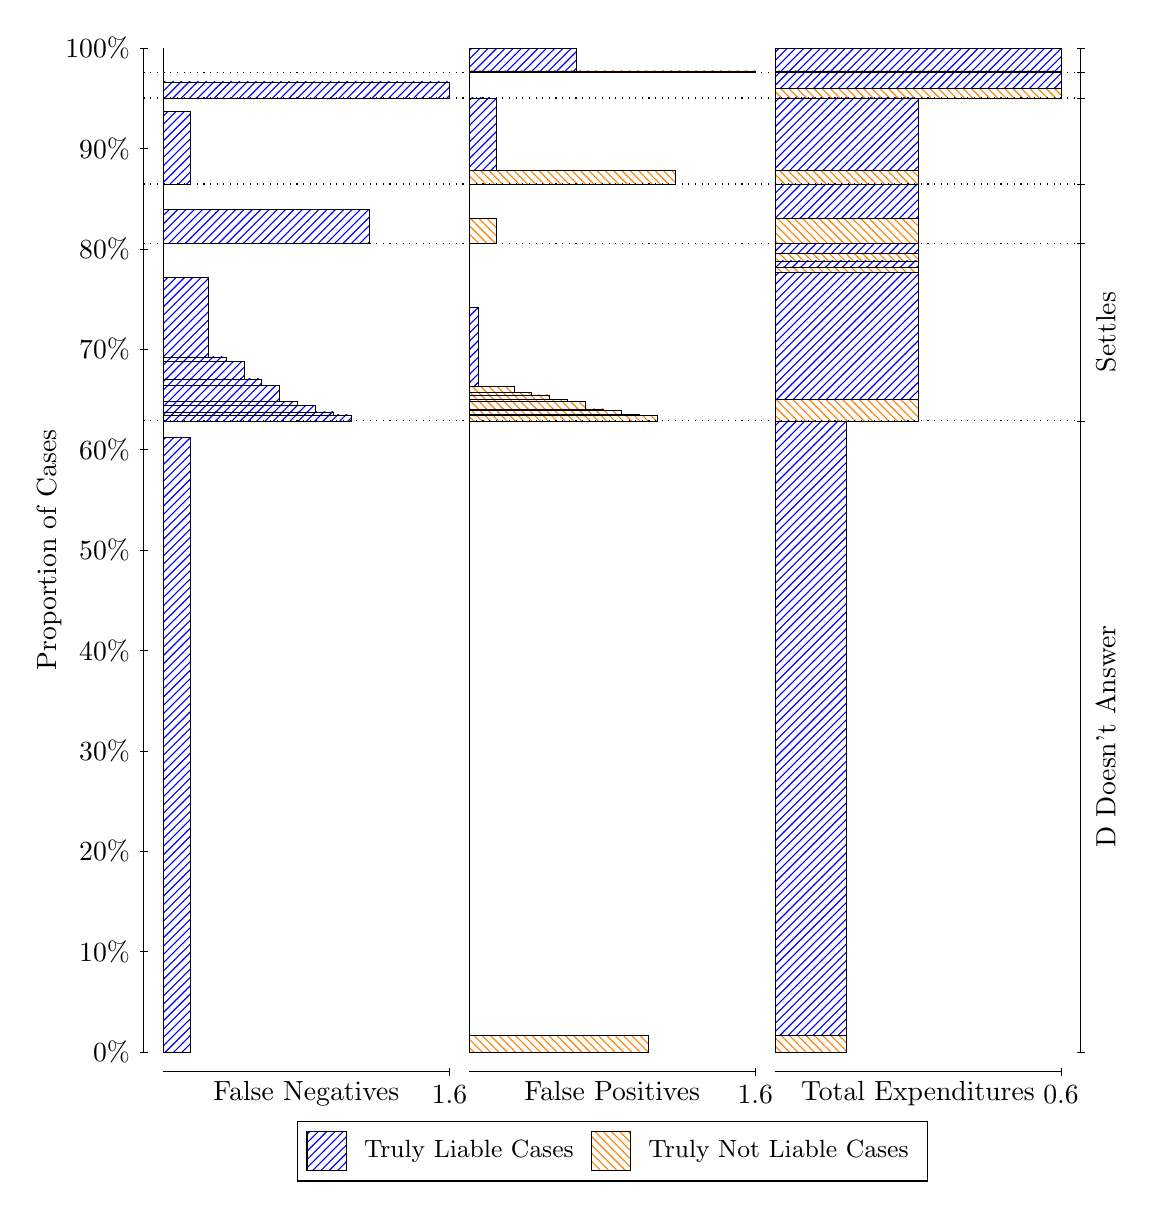
\begin{tikzpicture}
\draw[black, very thin] (1.5,1.75) -- (1.5,14.5);
\node[rotate=90, anchor=center] at (0.3, 8.125) {Proportion of Cases};
\draw[black, very thin] (1.45,1.75) -- (1.55,1.75);
\node[anchor=east] at (1.45, 1.75) {0\%};
\draw[black, very thin] (1.45,3.025) -- (1.55,3.025);
\node[anchor=east] at (1.45, 3.025) {10\%};
\draw[black, very thin] (1.45,4.3) -- (1.55,4.3);
\node[anchor=east] at (1.45, 4.3) {20\%};
\draw[black, very thin] (1.45,5.575) -- (1.55,5.575);
\node[anchor=east] at (1.45, 5.575) {30\%};
\draw[black, very thin] (1.45,6.85) -- (1.55,6.85);
\node[anchor=east] at (1.45, 6.85) {40\%};
\draw[black, very thin] (1.45,8.125) -- (1.55,8.125);
\node[anchor=east] at (1.45, 8.125) {50\%};
\draw[black, very thin] (1.45,9.4) -- (1.55,9.4);
\node[anchor=east] at (1.45, 9.4) {60\%};
\draw[black, very thin] (1.45,10.675) -- (1.55,10.675);
\node[anchor=east] at (1.45, 10.675) {70\%};
\draw[black, very thin] (1.45,11.95) -- (1.55,11.95);
\node[anchor=east] at (1.45, 11.95) {80\%};
\draw[black, very thin] (1.45,13.225) -- (1.55,13.225);
\node[anchor=east] at (1.45, 13.225) {90\%};
\draw[black, very thin] (1.45,14.5) -- (1.55,14.5);
\node[anchor=east] at (1.45, 14.5) {100\%};

\draw[black, very thin] (13.4,1.75) -- (13.4,14.5);
\draw[black, very thin] (13.35,1.75) -- (13.45,1.75);
\node[anchor=west] at (13.35, 1.75) {};
\draw[black, very thin] (13.35,9.764) -- (13.45,9.764);
\node[anchor=west] at (13.35, 9.764) {};
\draw[black, very thin] (13.35,12.022) -- (13.45,12.022);
\node[anchor=west] at (13.35, 12.022) {};
\draw[black, very thin] (13.35,12.773) -- (13.45,12.773);
\node[anchor=west] at (13.35, 12.773) {};
\draw[black, very thin] (13.35,13.866) -- (13.45,13.866);
\node[anchor=west] at (13.35, 13.866) {};
\draw[black, very thin] (13.35,14.188) -- (13.45,14.188);
\node[anchor=west] at (13.35, 14.188) {};
\draw[black, very thin] (13.35,14.5) -- (13.45,14.5);
\node[anchor=west] at (13.35, 14.5) {};

\draw[black, very thin, pattern color=blue, pattern=north east lines] (1.75,1.75) rectangle (2.0906,9.5566);
\draw[black, very thin, pattern color=orange, pattern=north west lines] (1.75,9.5566) rectangle (1.75,9.764);
\draw[black, very thin, pattern color=blue, pattern=north east lines] (1.75,9.764) rectangle (4.1344,9.8397);
\draw[black, very thin, pattern color=blue, pattern=north east lines] (1.75,9.8397) rectangle (3.9073,9.8798);
\draw[black, very thin, pattern color=blue, pattern=north east lines] (1.75,9.8798) rectangle (3.6802,9.9606);
\draw[black, very thin, pattern color=blue, pattern=north east lines] (1.75,9.9606) rectangle (3.4531,10.009);
\draw[black, very thin, pattern color=blue, pattern=north east lines] (1.75,10.009) rectangle (3.226,10.216);
\draw[black, very thin, pattern color=blue, pattern=north east lines] (1.75,10.216) rectangle (2.999,10.298);
\draw[black, very thin, pattern color=blue, pattern=north east lines] (1.75,10.298) rectangle (2.7719,10.52);
\draw[black, very thin, pattern color=blue, pattern=north east lines] (1.75,10.52) rectangle (2.5448,10.577);
\draw[black, very thin, pattern color=blue, pattern=north east lines] (1.75,10.577) rectangle (2.3177,11.585);
\draw[black, very thin, pattern color=orange, pattern=north west lines] (1.75,11.585) rectangle (1.75,12.022);
\draw[black, very thin, pattern color=blue, pattern=north east lines] (1.75,12.022) rectangle (4.3615,12.454);
\draw[black, very thin, pattern color=orange, pattern=north west lines] (1.75,12.454) rectangle (1.75,12.773);
\draw[black, very thin, pattern color=blue, pattern=north east lines] (1.75,12.773) rectangle (2.0906,13.695);
\draw[black, very thin, pattern color=orange, pattern=north west lines] (1.75,13.695) rectangle (1.75,13.866);
\draw[black, very thin, pattern color=blue, pattern=north east lines] (1.75,13.866) rectangle (5.3833,14.069);
\draw[black, very thin, pattern color=orange, pattern=north west lines] (1.75,14.069) rectangle (1.75,14.188);
\draw[black, very thin, pattern color=orange, pattern=north west lines] (1.75,14.188) rectangle (1.75,14.21);
\draw[black, very thin, pattern color=blue, pattern=north east lines] (1.75,14.21) rectangle (1.75,14.5);
\draw[black, very thin, pattern color=orange, pattern=north west lines] (5.6333,1.75) rectangle (7.9042,1.9574);
\draw[black, very thin, pattern color=blue, pattern=north east lines] (5.6333,1.9574) rectangle (5.6333,9.764);
\draw[black, very thin, pattern color=orange, pattern=north west lines] (5.6333,9.764) rectangle (8.0177,9.8297);
\draw[black, very thin, pattern color=orange, pattern=north west lines] (5.6333,9.8297) rectangle (7.7906,9.8431);
\draw[black, very thin, pattern color=orange, pattern=north west lines] (5.6333,9.8431) rectangle (7.5635,9.8945);
\draw[black, very thin, pattern color=orange, pattern=north west lines] (5.6333,9.8945) rectangle (7.3365,9.9182);
\draw[black, very thin, pattern color=orange, pattern=north west lines] (5.6333,9.9182) rectangle (7.1094,10.008);
\draw[black, very thin, pattern color=orange, pattern=north west lines] (5.6333,10.008) rectangle (6.8823,10.033);
\draw[black, very thin, pattern color=orange, pattern=north west lines] (5.6333,10.033) rectangle (6.8823,10.036);
\draw[black, very thin, pattern color=orange, pattern=north west lines] (5.6333,10.036) rectangle (6.6552,10.095);
\draw[black, very thin, pattern color=orange, pattern=north west lines] (5.6333,10.095) rectangle (6.4281,10.13);
\draw[black, very thin, pattern color=orange, pattern=north west lines] (5.6333,10.13) rectangle (6.201,10.201);
\draw[black, very thin, pattern color=blue, pattern=north east lines] (5.6333,10.201) rectangle (5.7469,11.209);
\draw[black, very thin, pattern color=blue, pattern=north east lines] (5.6333,11.209) rectangle (5.6333,12.022);
\draw[black, very thin, pattern color=orange, pattern=north west lines] (5.6333,12.022) rectangle (5.974,12.34);
\draw[black, very thin, pattern color=blue, pattern=north east lines] (5.6333,12.34) rectangle (5.6333,12.773);
\draw[black, very thin, pattern color=orange, pattern=north west lines] (5.6333,12.773) rectangle (8.2448,12.944);
\draw[black, very thin, pattern color=blue, pattern=north east lines] (5.6333,12.944) rectangle (5.974,13.866);
\draw[black, very thin, pattern color=orange, pattern=north west lines] (5.6333,13.866) rectangle (5.6333,13.985);
\draw[black, very thin, pattern color=blue, pattern=north east lines] (5.6333,13.985) rectangle (5.6333,14.188);
\draw[black, very thin, pattern color=orange, pattern=north west lines] (5.6333,14.188) rectangle (9.2667,14.21);
\draw[black, very thin, pattern color=blue, pattern=north east lines] (5.6333,14.21) rectangle (6.9958,14.5);
\draw[black, very thin, pattern color=orange, pattern=north west lines] (9.5167,1.75) rectangle (10.425,1.9574);
\draw[black, very thin, pattern color=blue, pattern=north east lines] (9.5167,1.9574) rectangle (10.425,9.764);
\draw[black, very thin, pattern color=orange, pattern=north west lines] (9.5167,9.764) rectangle (11.333,10.033);
\draw[black, very thin, pattern color=blue, pattern=north east lines] (9.5167,10.033) rectangle (11.333,11.65);
\draw[black, very thin, pattern color=orange, pattern=north west lines] (9.5167,11.65) rectangle (11.333,11.721);
\draw[black, very thin, pattern color=blue, pattern=north east lines] (9.5167,11.721) rectangle (11.333,11.797);
\draw[black, very thin, pattern color=orange, pattern=north west lines] (9.5167,11.797) rectangle (11.333,11.893);
\draw[black, very thin, pattern color=blue, pattern=north east lines] (9.5167,11.893) rectangle (11.333,12.022);
\draw[black, very thin, pattern color=orange, pattern=north west lines] (9.5167,12.022) rectangle (11.333,12.34);
\draw[black, very thin, pattern color=blue, pattern=north east lines] (9.5167,12.34) rectangle (11.333,12.773);
\draw[black, very thin, pattern color=orange, pattern=north west lines] (9.5167,12.773) rectangle (11.333,12.944);
\draw[black, very thin, pattern color=blue, pattern=north east lines] (9.5167,12.944) rectangle (11.333,13.866);
\draw[black, very thin, pattern color=orange, pattern=north west lines] (9.5167,13.866) rectangle (13.15,13.985);
\draw[black, very thin, pattern color=blue, pattern=north east lines] (9.5167,13.985) rectangle (13.15,14.188);
\draw[black, very thin, pattern color=orange, pattern=north west lines] (9.5167,14.188) rectangle (13.15,14.21);
\draw[black, very thin, pattern color=blue, pattern=north east lines] (9.5167,14.21) rectangle (13.15,14.5);
\draw[black, dotted] (1.5,9.764) -- (13.4,9.764);
\draw[black, dotted] (1.5,12.022) -- (13.4,12.022);
\draw[black, dotted] (1.5,12.773) -- (13.4,12.773);
\draw[black, dotted] (1.5,13.866) -- (13.4,13.866);
\draw[black, dotted] (1.5,14.188) -- (13.4,14.188);
\draw[black, very thin] (1.75,1.5) -- (5.3833,1.5);
\node[anchor=north] at (3.5667, 1.5) {False Negatives};
\draw[black, very thin] (5.3833,1.45) -- (5.3833,1.55);
\node[anchor=north] at (5.3833, 1.45) {1.6};

\draw[black, very thin] (5.6333,1.5) -- (9.2667,1.5);
\node[anchor=north] at (7.45, 1.5) {False Positives};
\draw[black, very thin] (9.2667,1.45) -- (9.2667,1.55);
\node[anchor=north] at (9.2667, 1.45) {1.6};

\draw[black, very thin] (9.5167,1.5) -- (13.15,1.5);
\node[anchor=north] at (11.333, 1.5) {Total Expenditures};
\draw[black, very thin] (13.15,1.45) -- (13.15,1.55);
\node[anchor=north] at (13.15, 1.45) {0.6};

\node[black, centered, rotate=90] at (13.72, 5.757) {D Doesn't Answer};
\node[black, centered, rotate=90] at (13.72, 10.893) {Settles};





\draw (7.449999999999999,1.5) node[draw=none] (baseCoordinate) {};
\begin{scope}[align=center]
        \matrix[scale=0.5, draw=black, below=0.5cm of baseCoordinate, nodes={draw}, column sep=0.1cm]{
            \node[rectangle, draw, minimum width=0.5cm, minimum height=0.5cm, pattern=north east lines, pattern color=blue] {}; &
            \node[draw=none, font=\small] (B) {Truly Liable Cases}; &
            \node[rectangle, draw, minimum width=0.5cm, minimum height=0.5cm, pattern=north west lines, pattern color=orange] {}; &
            \node[draw=none, font=\small] (B) {Truly Not Liable Cases}; \\
            };
\end{scope}

\end{tikzpicture}
\end{document}